% Created 2023-12-12 Di 10:34
% Intended LaTeX compiler: pdflatex
\documentclass[11pt]{article}
\usepackage[utf8]{inputenc}
\usepackage[T1]{fontenc}
\usepackage{graphicx}
\usepackage{longtable}
\usepackage{wrapfig}
\usepackage{rotating}
\usepackage[normalem]{ulem}
\usepackage{amsmath}
\usepackage{amssymb}
\usepackage{capt-of}
\usepackage{hyperref}
\usepackage[a4paper,width=160mm,top=25mm,bottom=25mm]{geometry}
\usepackage[style=authoryear]{biblatex}
\usepackage{lmodern} % Ensures we have the right font
\usepackage[T1]{fontenc}
\usepackage[utf8]{inputenc}
\usepackage{graphicx}
\usepackage{amsmath, amsthm, amssymb}
\usepackage[table, xcdraw]{xcolor}
\usepackage{float}
\hypersetup{hidelinks}
\definecolor{bblue}{HTML}{0645AD}
\usepackage[explicit]{titlesec}
\setlength{\parindent}{0pt}
\setlength{\parskip}{1em}
\usepackage{titling}
\setlength{\droptitle}{-6em}
\pretitle{\begin{center}\fontsize{20pt}{20pt}\selectfont}
\posttitle{\par\end{center}}
\preauthor{\begin{center}\vspace{-6bp}\fontsize{14pt}{14pt}\selectfont}
\postauthor{\par\end{center}\vspace{-25bp}}
\predate{\begin{center}\fontsize{12pt}{12pt}\selectfont}
\postdate{\par\end{center}\vspace{0em}}
\titlespacing\section{0pt}{5pt}{0pt} % left margin, space before section header, space after section header
\titlespacing\subsection{0pt}{5pt}{0pt} % left margin, space before subsection header, space after subsection header
\titlespacing\subsubsection{0pt}{5pt}{0pt} % left margin, space before subsection header, space after subsection header
\usepackage{enumitem}
\setlist[itemize]{noitemsep, topsep=0pt}
\setlist{itemsep=-2pt} % or
\addbibresource{~/biblio/pop-gen.bib}
\addbibresource{~/biblio/pop-gen.bib}
\usepackage[a4paper,width=160mm,top=25mm,bottom=25mm]{geometry}
\usepackage[style=authoryear]{biblatex}
\usepackage{lmodern} % Ensures we have the right font
\usepackage[T1]{fontenc}
\usepackage[utf8]{inputenc}
\usepackage{graphicx}
\usepackage{amsmath, amsthm, amssymb}
\usepackage[table, xcdraw]{xcolor}
\usepackage{float}
\hypersetup{hidelinks}
\definecolor{bblue}{HTML}{0645AD}
\usepackage[explicit]{titlesec}
\setlength{\parindent}{0pt}
\setlength{\parskip}{1em}
\usepackage{titling}
\setlength{\droptitle}{-6em}
\pretitle{\begin{center}\fontsize{20pt}{20pt}\selectfont}
\posttitle{\par\end{center}}
\preauthor{\begin{center}\vspace{-6bp}\fontsize{14pt}{14pt}\selectfont}
\postauthor{\par\end{center}\vspace{-25bp}}
\predate{\begin{center}\fontsize{12pt}{12pt}\selectfont}
\postdate{\par\end{center}\vspace{0em}}
\titlespacing\section{0pt}{5pt}{0pt} % left margin, space before section header, space after section header
\titlespacing\subsection{0pt}{5pt}{0pt} % left margin, space before subsection header, space after subsection header
\titlespacing\subsubsection{0pt}{5pt}{0pt} % left margin, space before subsection header, space after subsection header
\usepackage{enumitem}
\setlist[itemize]{noitemsep, topsep=0pt}
\setlist{itemsep=-2pt} % or
\addbibresource{~/biblio/pop-gen.bib}
\usepackage[a4paper,width=160mm,top=25mm,bottom=25mm]{geometry}
\usepackage[style=authoryear]{biblatex}
\usepackage{lmodern} % Ensures we have the right font
\usepackage[T1]{fontenc}
\usepackage[utf8]{inputenc}
\usepackage{graphicx}
\usepackage{amsmath, amsthm, amssymb}
\usepackage[table, xcdraw]{xcolor}
\usepackage{float}
\hypersetup{hidelinks}
\definecolor{bblue}{HTML}{0645AD}
\usepackage[explicit]{titlesec}
\setlength{\parindent}{0pt}
\setlength{\parskip}{1em}
\usepackage{titling}
\setlength{\droptitle}{-6em}
\pretitle{\begin{center}\fontsize{20pt}{20pt}\selectfont}
\posttitle{\par\end{center}}
\preauthor{\begin{center}\vspace{-6bp}\fontsize{14pt}{14pt}\selectfont}
\postauthor{\par\end{center}\vspace{-25bp}}
\predate{\begin{center}\fontsize{12pt}{12pt}\selectfont}
\postdate{\par\end{center}\vspace{0em}}
\titlespacing\section{0pt}{5pt}{0pt} % left margin, space before section header, space after section header
\titlespacing\subsection{0pt}{5pt}{0pt} % left margin, space before subsection header, space after subsection header
\titlespacing\subsubsection{0pt}{5pt}{0pt} % left margin, space before subsection header, space after subsection header
\usepackage{enumitem}
\setlist[itemize]{noitemsep, topsep=0pt}
\setlist{itemsep=-2pt} % or
\addbibresource{~/biblio/pop-gen.bib}
\usepackage[a4paper,width=160mm,top=25mm,bottom=25mm]{geometry}
\usepackage[style=authoryear]{biblatex}
\usepackage{lmodern} % Ensures we have the right font
\usepackage[T1]{fontenc}
\usepackage[utf8]{inputenc}
\usepackage{graphicx}
\usepackage{amsmath, amsthm, amssymb}
\usepackage[table, xcdraw]{xcolor}
\usepackage{float}
\hypersetup{hidelinks}
\definecolor{bblue}{HTML}{0645AD}
\usepackage[explicit]{titlesec}
\setlength{\parindent}{0pt}
\setlength{\parskip}{1em}
\usepackage{titling}
\setlength{\droptitle}{-6em}
\pretitle{\begin{center}\fontsize{20pt}{20pt}\selectfont}
\posttitle{\par\end{center}}
\preauthor{\begin{center}\vspace{-6bp}\fontsize{14pt}{14pt}\selectfont}
\postauthor{\par\end{center}\vspace{-25bp}}
\predate{\begin{center}\fontsize{12pt}{12pt}\selectfont}
\postdate{\par\end{center}\vspace{0em}}
\titlespacing\section{0pt}{5pt}{0pt} % left margin, space before section header, space after section header
\titlespacing\subsection{0pt}{5pt}{0pt} % left margin, space before subsection header, space after subsection header
\titlespacing\subsubsection{0pt}{5pt}{0pt} % left margin, space before subsection header, space after subsection header
\usepackage{enumitem}
\setlist[itemize]{noitemsep, topsep=0pt}
\setlist{itemsep=-2pt} % or
\addbibresource{~/biblio/pop-gen.bib}
\author{Philip L. Wolper}
\date{\today}
\title{Population Structure and Genetic Variation of \emph{Plasmodium falciparum} in West and Central Africa\\\medskip
\large TUM, Section of population genetics, Prof. Aureli\'{e}n Tellier \linebreak Research internship final report, WS 2023}
\hypersetup{
 pdfauthor={Philip L. Wolper},
 pdftitle={Population Structure and Genetic Variation of \emph{Plasmodium falciparum} in West and Central Africa},
 pdfkeywords={},
 pdfsubject={},
 pdfcreator={Emacs 27.1 (Org mode 9.6.7)}, 
 pdflang={English}}
\begin{document}

\maketitle
\begin{abstract}
This report presents insights on the genetic diversity and population structure of the malaria-causing parasite \emph{Plasmodium falciparum} using whole-genome SNP data from various African countries. We confirm previous knowledge of high admixture and limited population substructure between African countries. Our \emph{de novo} clustering analysis generally confirms this. Interestingly, we find chromosome 11, to exhibit higher signatures of isolation-by-distance than chromosome 2. Additionally, we calculate the unfolded site-frequency spectrum (SFS) for both chromosomes and show it to be U-shaped. We provide some discussion on evolutionary mechanisms leading this U-shaped SFS in \emph{P. falciparum} and emphasize how population genetics, particularly multiple-merger coalescents, can be applied to understand the evolutionary dynamics of \emph{P. falciparum} in the future, contributing to better malaria control and drug intervention strategies.
\end{abstract}

\section*{Introduction}
\label{sec:org0e8bf3c}
\emph{Plasmodium falciparum}, an apicomplexan human parasite and the most important disease agent of malaria, is a major global health threat, with nearly half the worlds population at risk for the disease. Especially tropical and subtropical regions suffer the highest disease burden, and nearly 95\% of all cases and deaths occur in Africa. Fatalities in this region mainly affect young children, as 80\% of malaria mortality occurs in children aged 5 years or younger (\cite{world2022world}). Although impoved control measures have contributed to a steady decline of malaria cases and death rates over the past 20 years, increasing resistances to major anti-malaria drugs, such as artemisin and chloroquinine, are constantly threatening to undermine eradication progress of the disease. Continued effective malaria control measures, rely on disentangling the effects of population structure, selection, recombination and random processes on genome evolution and population dynamics.

Understanding the genetic diversiy and population structure of \emph{P. falciparum} is crucial to make valid inferences of selection on parasite traits, such as drug resistance. This allows us to seperate adaptive changes in parasite allele frequencies from non-adaptive changes. Importantly, conclusions about selective processes require comprehensive evolutionary 'null'-models, to test hypothesis. Such models should account for population structure, demographic history, as well as other biological or life-history traits, that could potentially lead to signatures of genetic variation similar to selection. Therefore it is important to assess the structure of a sampled parasite population when making further inferences about adaption.

The population genetic structure of \emph{P. falciparum} has been shown to vary greatly when looking at different global regions, and is closely associated with transmission intensity and disease epidemiology (\cite{anderson-2000-micros-marker}). Regions with low transmission, such as South America or South East Asia, typically show low levels of multiple co-infection, leading to predominantly clonal populations, with low genetic diversity and high levels of linkage disequilibrium (LD). This LD often results from epidemic expansion of a particular clone. On the other hand, high levels of parasite transmission, such as in malaria endemic regions across Africa, leads to high levels of co-infection in the host, high rates of outcrossing and rapid decay in LD (\cite{mu-2005-recom-hotsp}). This variation of population genetic structure makes generalized studies about evolutionary patterns in \emph{P. falciparum} difficult to conduct and interpret reliably.

Most population genetics inferences are based on the Wright-Fisher model and Kingman coalescent framework to connect the population genetic theory to real-world population genetics data (eg. \cite{li-2013-coales-tree}). In order to assess the genetic variation in a population, summary statistics can be calculated. One such commonly used statistics is the site frequency spectrum (SFS), a histogram of allele frequencies in the population. Neutral theory predicts most allelic variants expected to be rare, because they do not influence an oranisms fitness and will be lost by genetic drift. For a panmictic population, the expected SFS for can be calculated, using coalescent model simulations following the assumptions of Wright-Fisher populations. Typically, the observed SFS spectrum differs from the expected ones, and the type of this skew can reveal details about selective or demographic processes occuring in the population. For example, an excess in rare variants (such as singletons), can be interpreted as signals of positive or negative selection or population expansion.

In nature many SFS are observed to be U-shaped (uSFS) (\cite{freund-2023-inter-pervas}), with an excess of rare and common derived alleles. One common explaination for the uSFS is positive selection at several loci with neutral variants hitchhiking to high-frequencies as well (\cite{bustamante-2001-direc-selec}). This phenoma is predicted to be reinforced by temporally fluctuating selection (\cite{huerta-sanchez-2008-popul-genet}). Many other alternative explaination for a uSFS have been proposed, such as gene flow from non-sampled populations (\cite{marchi-2020-gene-flow}), population subdivision (\cite{lapierre-2016-impac-selec}), biased gene conversion (\cite{pouyet-2018-backg-selec}), misorientation of ancestral and derived alleles (\cite{baudry-2003-effec-misor}) and well as various reproductive strategies (\cite{tellier-2014-coales}).

This great number of factor affecting SFS distributions can make it difficult to effectively identify which forces are dominantly acting on the evolution of an organism. While the Kingman coalescent models can deal with many different assumption such as population structure or changes in population size, it is less suited to deal with large variances in offspring numbers (sweepstake reproduction) and merging of more than two lineages. Sweepstake reproduction applies to species, which produce a high number of offspring together with high early-life mortality, leading to a very recent common ancestor. Similarly, strong and recurrent selective sweeps can lead to the coalescence of multiple branches in the genealogies simultaneously. Because of the limitations the Kingman coalescent is faced with regarding the such life-history traits, species violating these assumptions are better modelled with a more class of coalescent models using multiple merger coalescents (MMC) (\cite{tellier-2014-coales}). Genealogies originating from MMC models, have been observed across all kingdoms of life (\cite{freund-2023-inter-pervas}). Inferences methods based on the classical Wright-Fisher assumptions can lead to erroneous interpretations of different evolutionary mechanisms, if applied to species with strong multiple merger phenomena. Thus for organism with life-cycles that produce MMC genealogies, such as many pathogens or marine organisms, multiple-merger coalescent models have been recommended for inferring the expected SFS (\cite{freund-2023-inter-pervas}).

In this report we analyze population structure and genetic variation of \emph{Plasmodium falciparum} in select African countries. We calculate the unfolded site-frequency spectrum of the population and provide some context to interpret it in.
\section*{Data and Methods}
\label{sec:org82bf919}
In this section, we provide a comprehensive overview of the data source, data preprocessing steps, and the analytical methods employed for this investigation.

\subsection*{Pf7 data availability}
\label{sec:orge89be26}
The analysis of population genetics data for \emph{Plasmodium falciparum} presented in this report was derived from whole-genome Single Nucleotide Polymorphism (SNP) data. The dataset used in this study was obtained from the MalariaGEN Pf7 data resource, a large release of genome variation data from \emph{Plasmodium falciparum} (\cite{MalariaGEN-2023-pf7}). In whole, Pf7 consists of over 16,000 samples high-quality from over 33 countries and 82 partner studies. By using a method called selective whole genome amplification (sWGA) prior to sequencing, samples could be collected from dried blood spots. While showing the use of sWGA does not indroduce any biases in coverage or population structure, the Pf7 resource is the largest publicly available resource for genomic information of \emph{P.falciparum}. Pf7 provides data on genomic variation as variant calling format (VCF) files per chromosome. The vcf files are freely available from an FTP server using an FTP client (\url{ftp://ngs.sanger.ac.uk/production/malaria/Resource/34/Pf7\_vcf/}).

\subsection*{Data}
\label{sec:orgeb03b20}
For this report, we chose to analyze 1846 sample from 4 different african countries: Democratic Republik of Congo (DRC), The Gambia, Kenya and Tanzania. The number of samples per country is 520, 452, 285 and 598, respectively and all of them come from 2010-2017, never more than 4 years for any given country. Because of the size of the data, our analysis was conducted for chromosomes 2 and 11, which we downloaded from the FTP server.

\subsection*{Filtering and processing}
\label{sec:org3643fd9}
Filtering steps and manipulation of the vcf files were done using the software \emph{bcftools} (\cite{danecek-2021-twelv-years}). The VCF files for chromosomes 2 and 11 were filtered to include only biallelic SNPs, which where designated with the filter 'PASS' by the Pf7 data resource. Additionally, we retained only the SNPs with a quality score VQSLOD > 5.0. In total this yielded data sets with 16,269 and 44,040 SNPs, for chromosomes 2 and 11, respectively.
The proportion of heterozygous genotypes in the VCF files was relatively small: 0.2\% and 0.3\% for chromosome 2 and 11, respectively. To avoid possible effects of multiple infection, we removed all heterozygous genotypes (including both phased and unphased GT fields), by setting them to missing data (./.).

\subsection*{Population genetics statisics}
\label{sec:org0496f6d}
Basic population genetic measures, such as \(\theta\) or Tajima' D statistic, were calculated using the R package \emph{PopGenome} (\cite{pfeifer-2014-popgen}). Statistics were calculated in sliding windows of 10 Kb for both chromosomes. Additionally, we calculated calculated recombination events accross each chromosome, according to the four-gamete test, also implemented in \emph{PopGenome}.

\subsection*{Population structure}
\label{sec:org7f50f99}
Local Population structure of the selected data was investigated using discriminant analysis of principal components (dapc), performed using the R package \emph{adegenet} (\cite{jombart-2010-discr-analy}). The dapc analysis was conducted according to the guidelines outlined by \cite{thia-2022-guidel-stand}. To determine the number of clusters suited for discrimination, we performed a K-means clustering algorithm prior to the dapc using \emph{adegenet}'s in-built function \emph{find.clusters()}. The K-means algorithm implemented in \emph{find.cluster()} uses proir tranformation by principal component analysis (PCA), retaining principal component axis which approximately 80-90\% of the variance in the data set. The number of clusters to be used for the dapc was selected based on the Bayesian Information Criterion (BIC). The dapc analysis was run with K-1 PCA axes and K-1 discriminant axes, using the K-mean group assignments as priors.

Extending the dapc analysis, we did a population structure analysis using the software \emph{ADMIXTURE} (\cite{alexander-2009-fast-model}). The VCF files had their chromosome renamed numerically and using \emph{plink2} we converted them to .bed files. We conducted admixture analysis for a wide range of K values, including the value used for the dapc. The results of the admixture analysis were validated by comparing the CV error values of each run of K.

\subsection*{Site-frequency spectrum}
\label{sec:org06d2de7}
In order to calculate an unfolded site-frequency spectrum for the SNP data, we used \emph{Plasmodium reichenowi} as an outgroup. The genome assembly \emph{PrCDC} of \emph{P.reichenowi} was obtained from (\url{ftp://ftp.sanger.ac.uk/pub/project/pathogens/reichenowi/2018/October\_2018}). Since the PrCDC assembly was assembled by using the \emph{Plasmodium falciparum} Pf7 in a refernce guided assembly, we compare the two using genome alignment. We aligned the \emph{P.falciparum} reference genome (Pf7) with the \emph{P.reichowi} reference (PrCDC) using \emph{mummer4} (\cite{marcais-2018-mummer}), and extracted the segregating sites between both assemblies. Using an R script (\url{https://taylorreiter.github.io/2019-05-11-Visualizing-NUCmer-Output/}), we plotted the mapping coverage to ensure sufficient overlap between the genomes (Fig. \ref{nucmer_coverage_chr2} and \ref{nucmer_coverage_chr11})

To polarize the SNPs found in the Pf7 VCF data set, we compare the segregating sites between out Pf7 refernce and the outgroup with the polymorphic sites found in the vcf file. From the genome alignment we found 927 and 2082 segregating positions, respectively for chromosome 2 and 11, which were also found to be polymorphic in the \emph{P.falciparum} data set. Of these, 524 and 1207 SNPs, respectively, had an alternative (ALT) alleles matching the allele found in the outgroup. These SNPs had their alternative allel redesignated as the anchestral allele, while the reference allele is assumed to be the 'new' alternative (derived) allele. For sites, that were not segregating between the reference and the outgroup, polarisation cannot be performed, and we assume the reference allele to be anchestral. The idea is that the allele found on the outgroup can be considered the anchestral allele if it matches an allele found in the \emph{P. falciparum} population, because the probability of the same allele arising in the outgroup and our population is very small under the infinte-sites model.

After each allele recieved a designation of anchestral or derived, we removed sites, that either had no alternative allele or a fixed alternative allele, since these would skew the site-frequency spectrum. Additionally, we divided the number of allele counts and total counts by two to reflect the haploid nature of \emph{P.falciparum}. This resulted in final sets of 5399 and 13847 SNPs, respectively for chromosome 2 and 11, which could be used to plot the unfolded site-frequency spectrum.
\section*{Results}
\label{sec:orgc32c3bf}
Across both chromosomes analyzed, we found that diversity statisic, such as \(\theta\)\textsubscript{W}, \(\theta\)\textsubscript{pi}, the number of segregating sites S and Tajima's D to vary quite a lot (Fig. \ref{div_stats_chr2} and \ref{div_stats_chr11}), as is to be expect from different regions of the genome. Interestingly, we found overall very low values of Tajima's D across all samples (Fig. \ref{div_stats_chr2}A and \ref{div_stats_chr11}A). When comparing the nucleotide diversity measure of Watterson, \(\theta\)\textsubscript{W} to an estimate of recombination events Hudson-Kaplan-RM, we find a higher diversity for windows with more recombination events (Fig. \ref{div_stats_chr2}E and \ref{div_stats_chr11}E). This is expected under linked selection, where selection between linked loci will drag down polymorphism. Less linked regions with higher recombination frequencies, therefore are estimated to show more polymorphism. At high recombination rates, this effect, \(\theta\)\textsubscript{W} values flatten out, because polymorphism ultimately is constrained by mutation.

\begin{center}
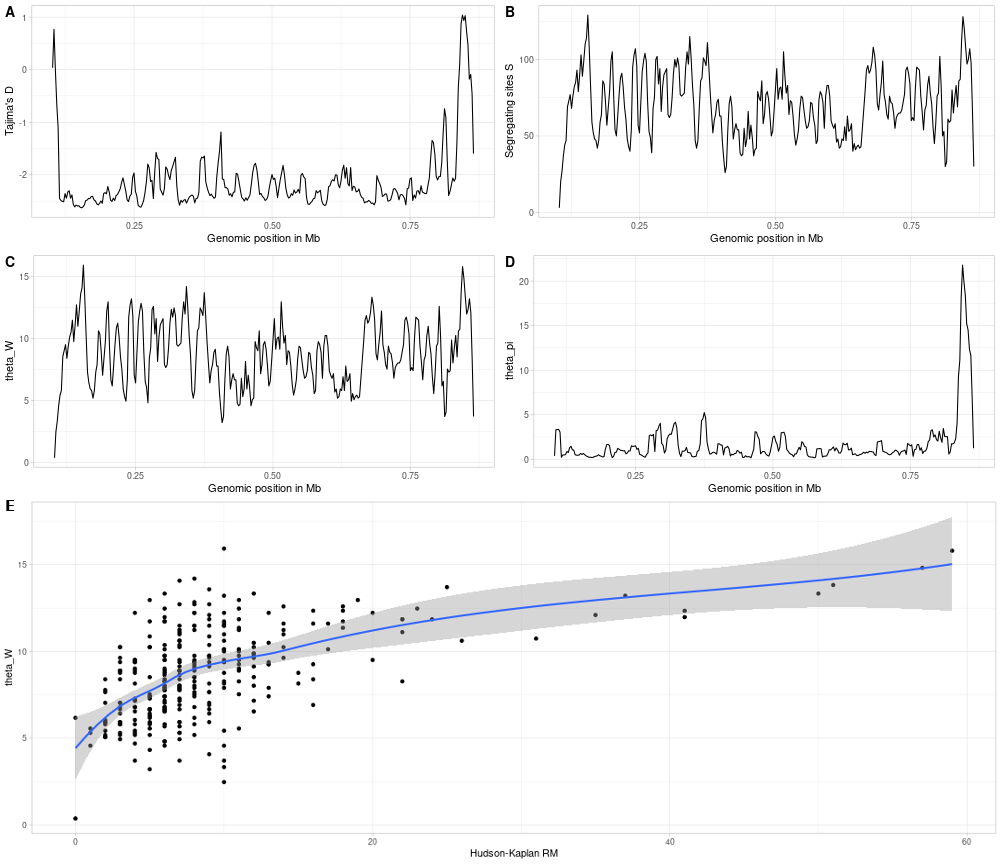
\includegraphics[width=0.6\textwidth]{./figures/stats_panel_chr2.png}
\captionof{figure}{\label{div_stats_chr2}Diversity statistics of chromosome 2, calculated in sliding windows of 10 Kb length. (A) Tajima's D, (B) Segregating sites S, (C) \(\theta\)\textsubscript{Watterson}, (D) \(\theta\)\textsubscript{pi} and (E) \(\theta\)\textsubscript{W} plotted against Hudson-Kaplan RM in 10 Kb windows.}
\end{center}

\begin{center}
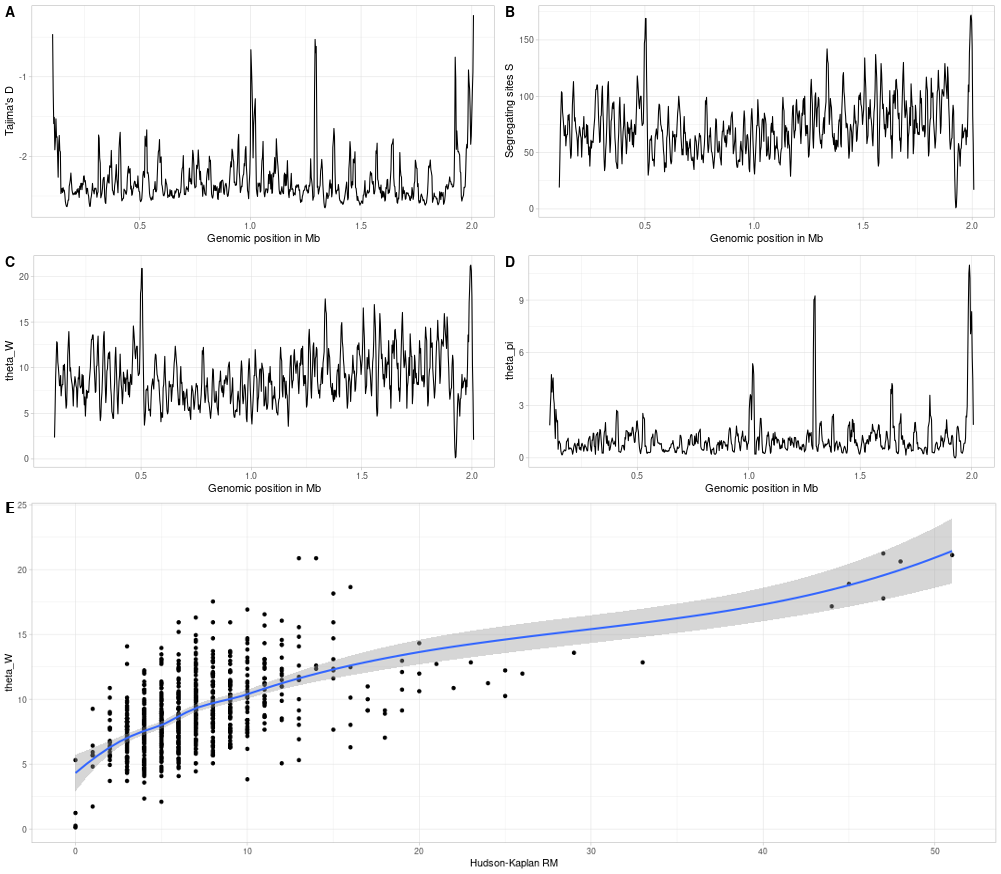
\includegraphics[width=0.6\textwidth]{./figures/stats_panel_chr11.png}
\captionof{figure}{\label{div_stats_chr11}Diversity statistics of chromosome 11, calculated in sliding windows of 10 Kb length. (A) Tajima's D, (B) Segregating sites S, (C) \(\theta\)\textsubscript{Watterson}, (D) \(\theta\)\textsubscript{pi} and (E) \(\theta\)\textsubscript{W} plotted against Hudson-Kaplan RM in 10 Kb windows.}
\end{center}

We conducted two parallel approaches to investigate possible population structure in our \emph{P. falciparum} samples, discriminant of principle components (dapc) and bayesian structure analysis using the software ADMIXTURE. We first chose to analyze if population structure follows the sampled locations, using these as our a priori labels. Generally we found high levels of admixture between populations, although we could observe some signals of geographic structuring (Fig. \ref{Pop_Struct_country_chr2} and \ref{Pop_Struct_country_chr11}). Specifically, the Gambian samples showed the most differentiation in the admixture analysis for the other locations. While the distruct plots of te structure analysis show similar low, but present population structure for both chromosomes, it is noteworthy, that chromosome 2 seems to have much less population structure than chromosome 11, as can be seen from the dapc (Fig. \ref{Pop_Struct_country_chr2}B) and (Fig. \ref{Pop_Struct_country_chr11}B).

\begin{center}
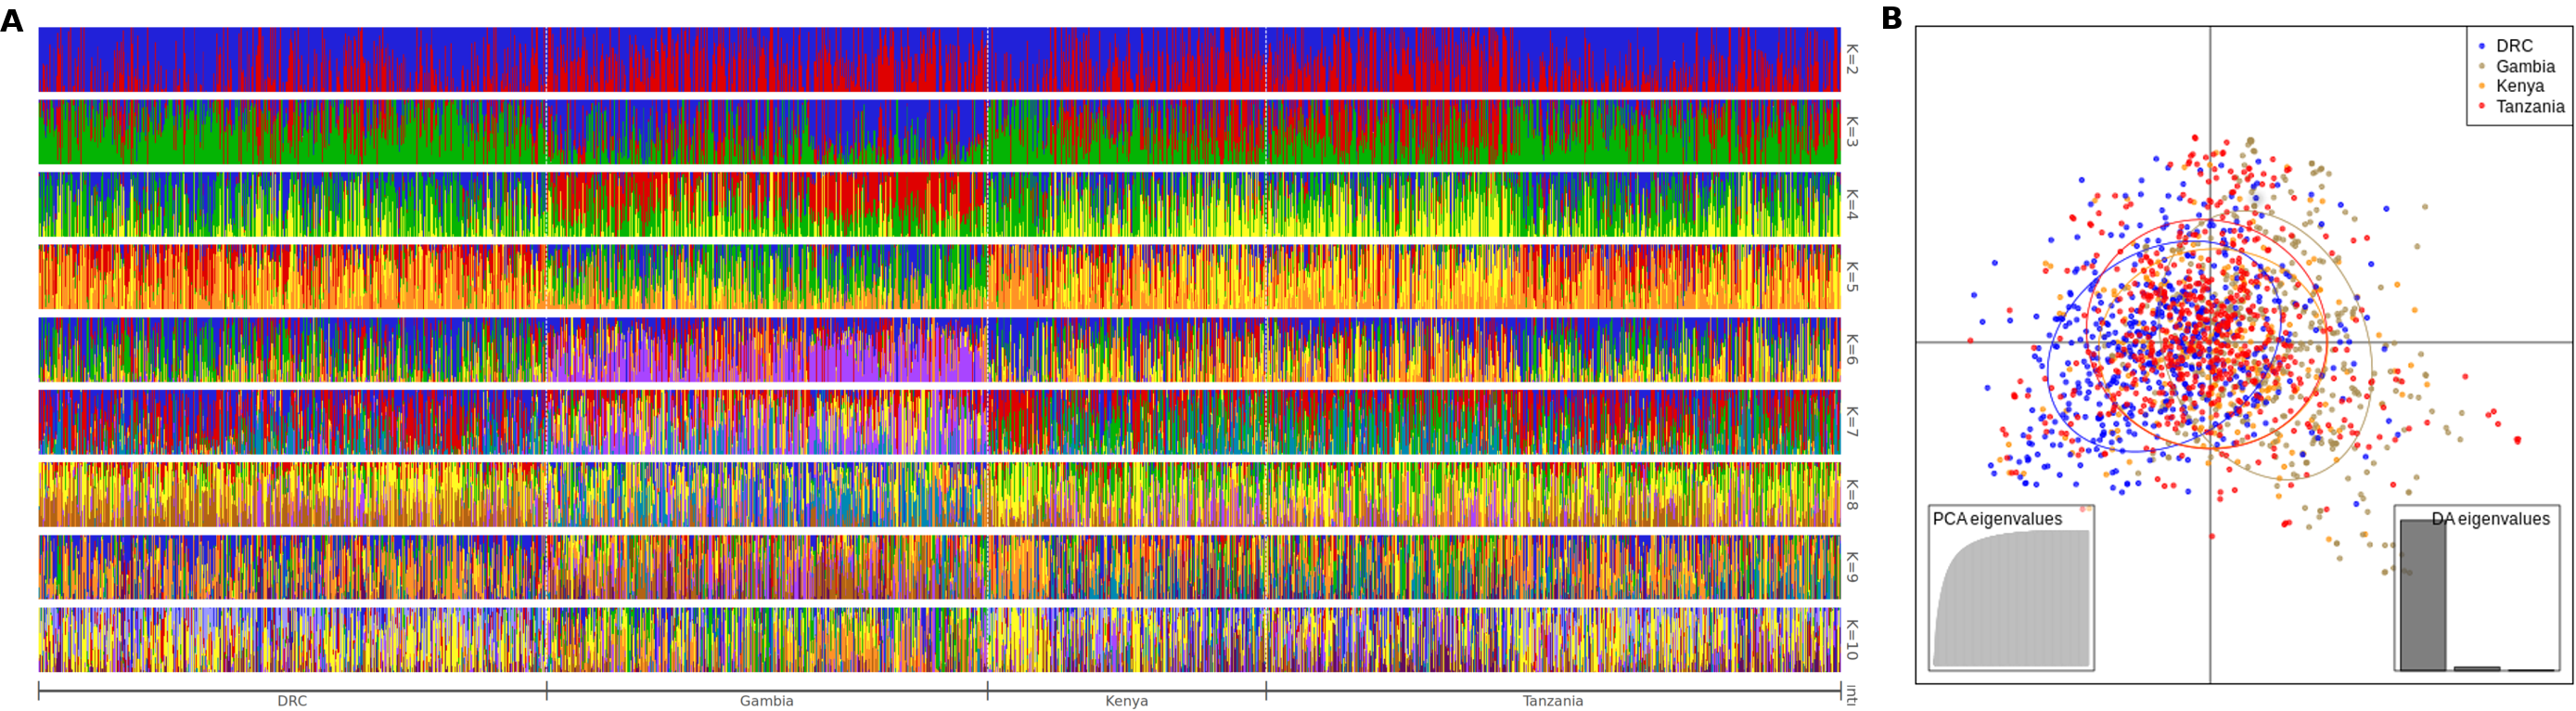
\includegraphics[width=1\textwidth]{./figures/Population_structure_countries_chr2.png}
\captionof{figure}{\label{Pop_Struct_country_chr2}Population structure analysis of \emph{P. falciparum} chromosome 2, showing the clustering by predefined labels based on sampling location.}
\end{center}

\begin{center}
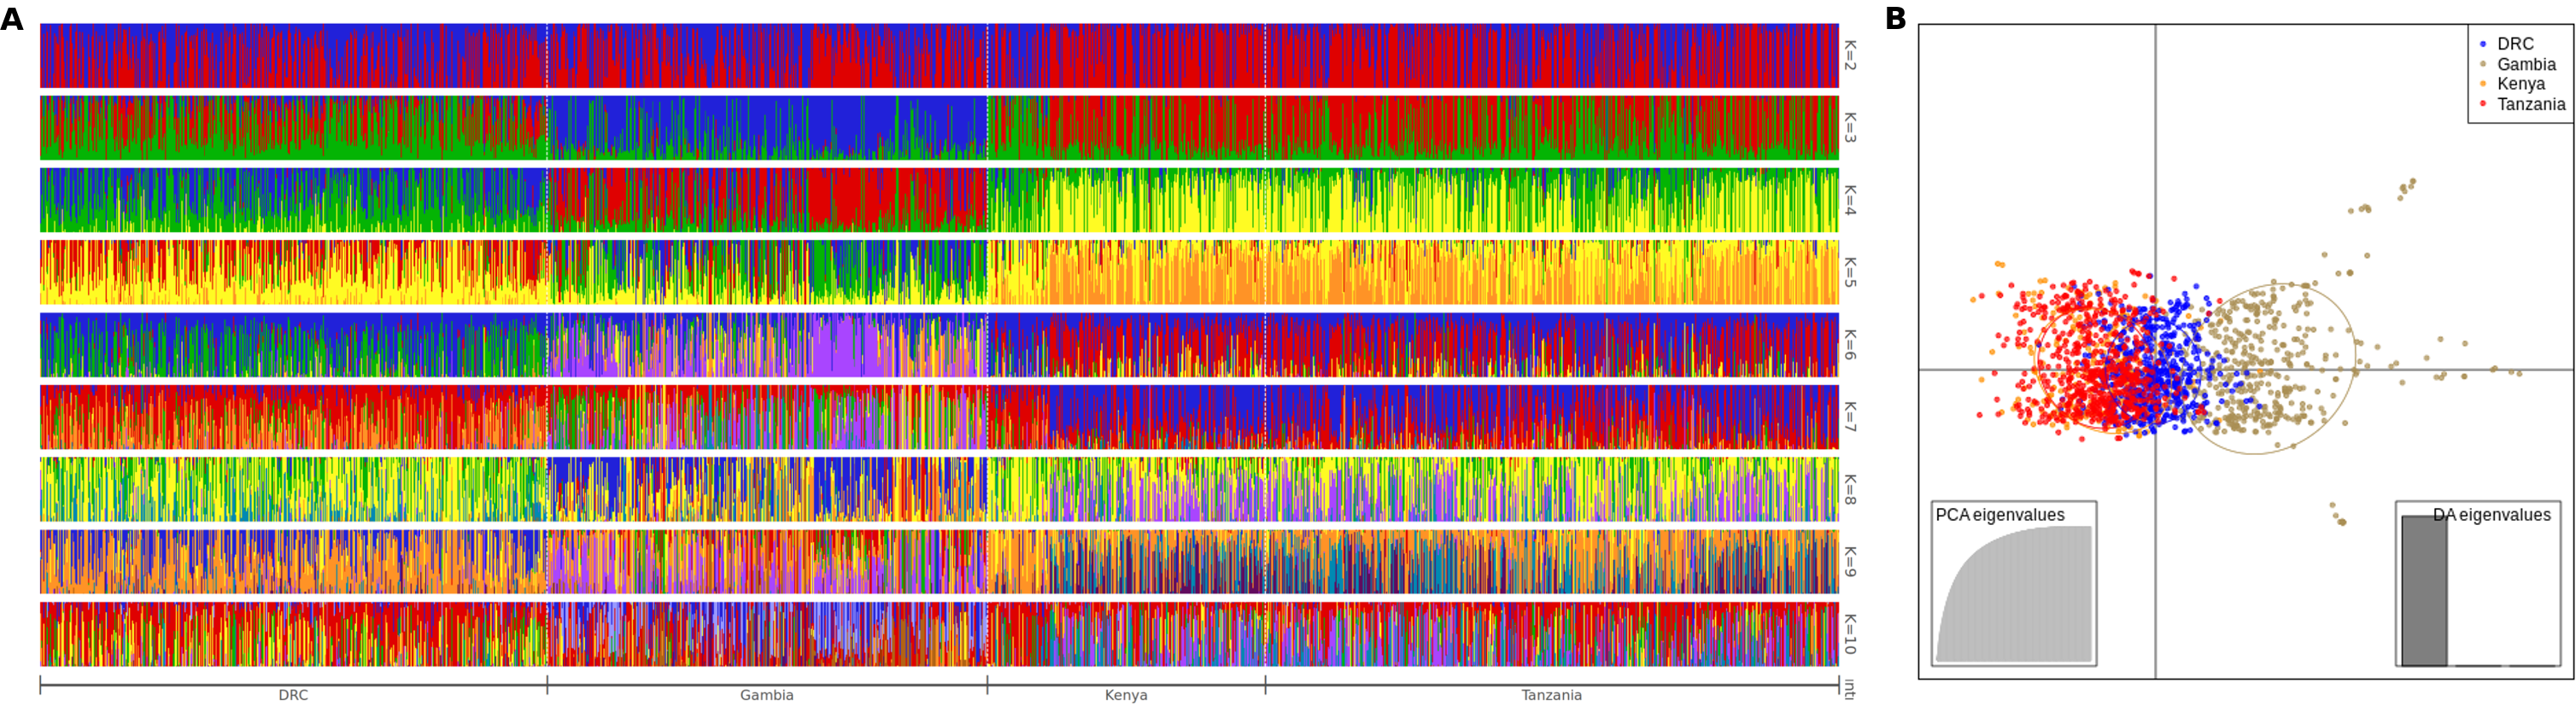
\includegraphics[width=1\textwidth]{./figures/Population_structure_countries_chr11.png}
\captionof{figure}{\label{Pop_Struct_country_chr11}Population structure analysis of \emph{P. falciparum} chromosome 11, showing the clustering by predefined labels based on sampling location.}
\end{center}

Next, we were interested in possible other causes of population structure in african \emph{P. falciparum} other than the geographic locations. We inferred the number of groups and membership \emph{de novo} using a K-means clustering algorithm, \emph{find.clusters()}, described in the dapc manual (\cite{jombart-2010-discr-analy}). The optimal value of K was determined to be 9 and 10, respectively for chromosome 2 and 11, significantly more than the a priori groups based on sampling location. We performed dapc analysis on these newly inferred groups, and clustering of both chromosomes into groups, but some of the clusters seem to overlap quite significantly. Chromosome 2 shows more distinct clustering by inferred group labels, than chromosome 11, but they do not correlate with the sampling location or year (Fig. \ref{dapc_corr_chr2}). In contrast, the inferred clusters of chromosome 11 seem to  correlate roughly with the sampling location and year. (Fig. \ref{dapc_corr_chr11}). When sorting the individuals in the admixture analysis by these inferred group labels, we found the results to agree with the dapc (Fig. \ref{admix_Kmeans}).

\begin{figure}[htbp]
\centering
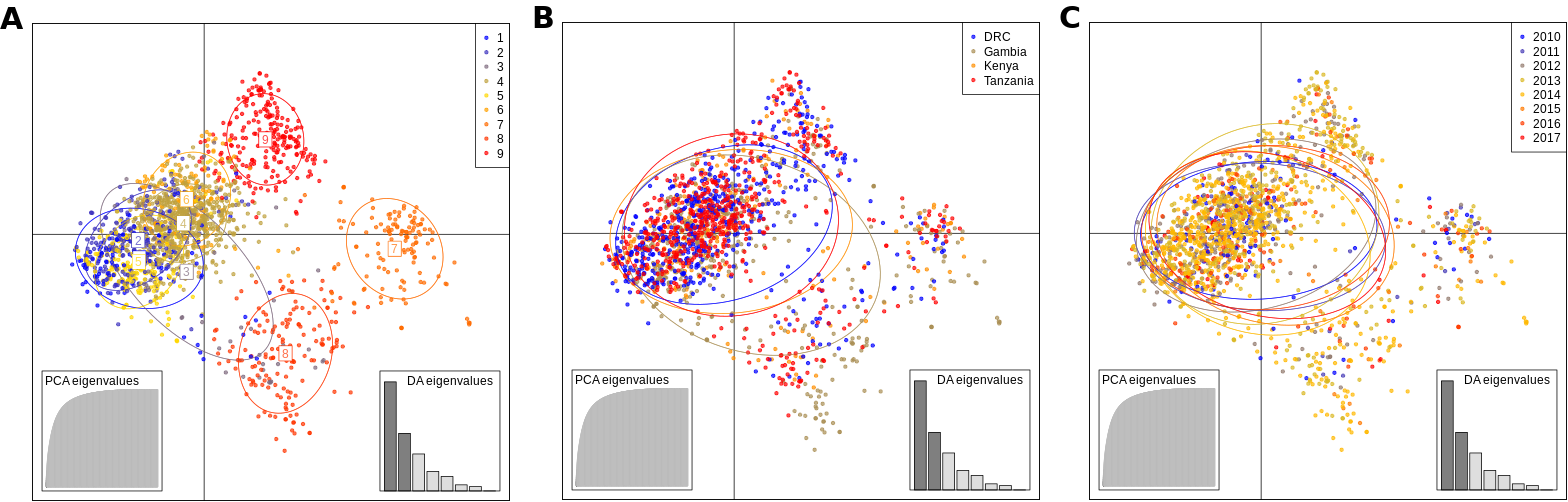
\includegraphics[width=0.9\textwidth]{./figures/dapc_Kmeans_chr2.png}
\caption{\label{dapc_corr_chr2}DAPC analysis of nine population clusters inferred \emph{de novo} with a K-means algorithm, chromosome 2. (A) Individuals colored according to assigned clusters. (B) Individuals colored by their sample location. (C) Individuals are colored by the sampled year.}
\end{figure}

\begin{figure}[htbp]
\centering
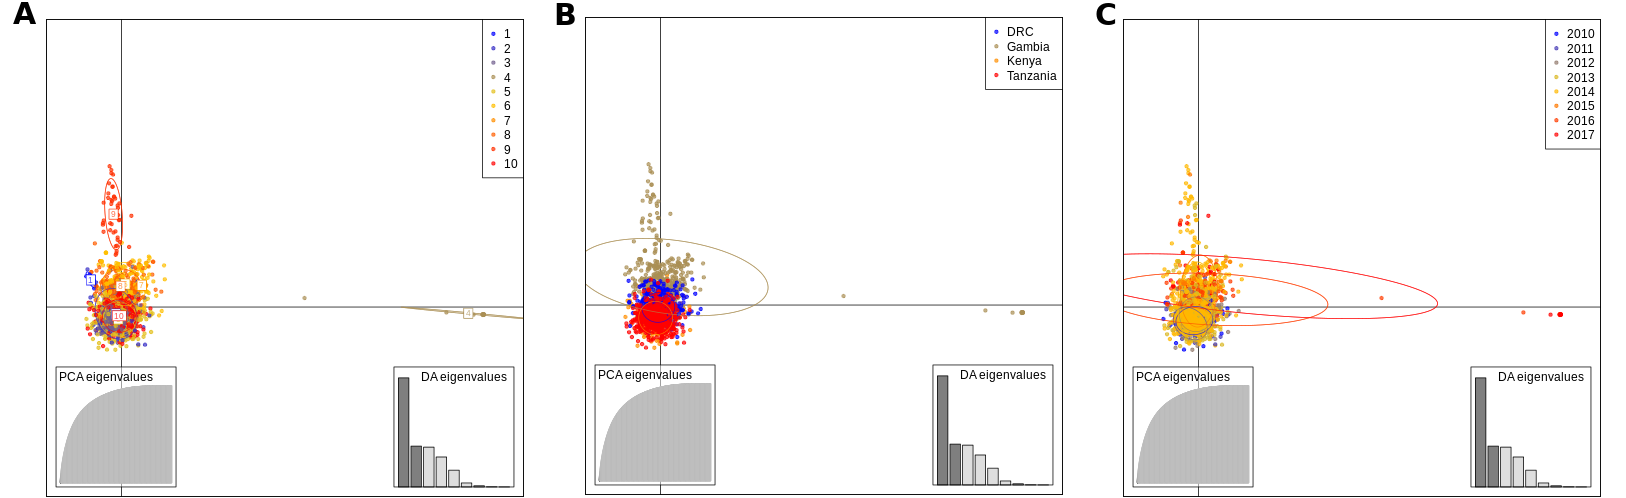
\includegraphics[width=0.9\textwidth]{./figures/dapc_Kmeans_chr11.png}
\caption{\label{dapc_corr_chr11}DAPC analysis of nine population clusters inferred \emph{de novo} with a K-means algorithm, chromosome 2. (A) Individuals colored according to assigned clusters. (B) Individuals colored by their sample location. (C) Individuals are colored by the sampled year.}
\end{figure}

In order to allow for more detailed inferences about the demographic history of the population and evolutionary forces such as selection we calculated the a polarized site frequency spectrum (SFS), for both chromosomes (Fig. \ref{SFS_unfolded}). The SFS we found, both had a U-shaped character, with an excess of singletons compared the the neutral expectation and increased high-frequency alleles. Because hidden population can influence the shape of the SFS, when samples from different populations are pooled together (\cite{lapierre-2016-impac-selec}), we calculated the SFS for samples from Gambia as well, as Gambia was the most distinct country from the others (Fig. \ref{SFS_gambia}). We found the U-shape in the Gambian SFS as well, which indicates the discovered U-shape is not due to unidentified substructuring of the sampled parasites.

\begin{figure}[htbp]
\centering
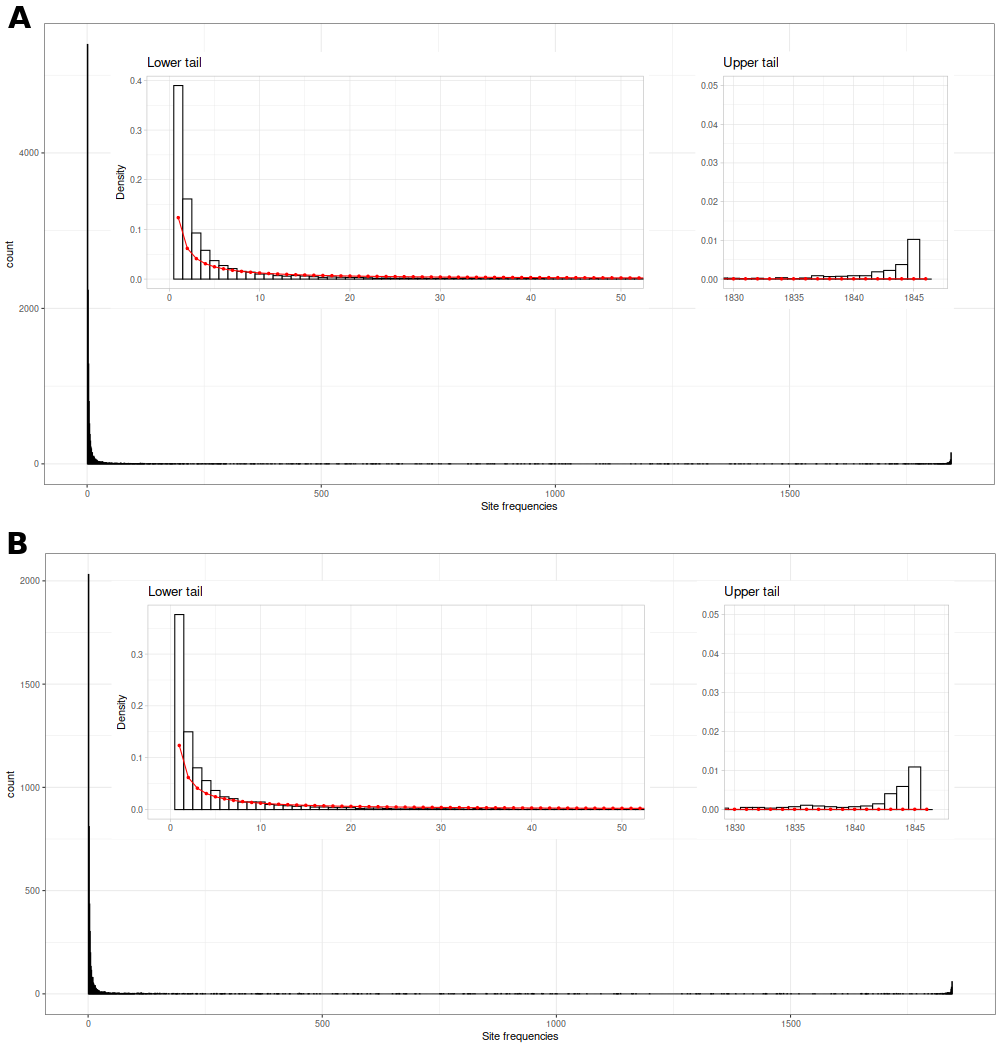
\includegraphics[width=0.67\textwidth]{./figures/sfs_unfolded_scaled.png}
\caption{\label{SFS_unfolded}Unfolded site frequency for chromosome 2 (A) and 11 (B).}
\end{figure}
\section*{Discussion}
\label{sec:org66bb4f3}
When calculating genome-wide levels of polymorphism, we found levels of both \(\theta\)\textsubscript{W} and pi to vary significantly for different regions of the genome. While this is expected due to varying levels of mutations and recombination, selection of certain genes and region is also a plausible explaination. It remains to be indentified if a significant proportion of putative genes under selection coincide with the observed regions of reduced polymorphism found. Furthermore, we found Tajima's D to vary across the genome, but generally being strongly negative for both chromosomes analyzed in each subpopulation separately, as well as for the total population. Negative values of Tajima's D across multiple chromosomes can be sign of population expansion, which would be consistent with findings of other studies (\cite{rich-2000-popul-struc}). This is likely linked to expansion of human populations and increased vectorial capacity since the last glacial maximum (\cite{donnelly-2001-eviden-recen}).

We investigated population structure in \emph{P. falciparum} samples from the African countries of Gambia, Democratic Republic of Congo, Kenya and Tanzania. Applying DAPC analysis, we found very little population structure, with samples from Gambia being the most differntiated in one of the two chromosomes, supporting a weak form of isolation by  distance, as Gambia is the most distant from the other three countries. It is feasible, that this relative lack of population structure is due to strong migration from humans, as human movement has shown to influence parasite movement at smaller geographic scale in Kenya and Uganda (\cite{nderu-2019-genet-diver}).

Complementing the DAPC analysis, we performed ADMIXTURE analysis, and found high levels of admixture between all subpopulations of \emph{P. falciparum}. These results can be interpreted in the context of high malaria transmission leading to increased recombination between different strains during co-infection (\cite{anderson-2000-micros-marker}). It remains to be investigated, how recombination rates correlate with levels of within-host diversity F\textsubscript{WS} and genome-wide linkage disequilibrium.

We assigned ancestral states using the outgroup species \emph{P. reichenowi} and calculated the unfolded site-frequency spectrum (SFS) for chromosomes 2 and 11. The number of SNPs we were able to polarize, was limited to divergent sites between the outgroup and ingroups which were segregating in \emph{P.falciparum}.  While we deem our method of assigning ancestral states to allels to be robust under the infinite-sites model, we acknowledge misorientations could happen due incomplete lineage sorting and sites not fully diverged between the two parasite species or recurrent mutation at the same site (i.e. homplasy) (\cite{baudry-2003-effec-misor}). Including more samples of the outgroup can increase the certainty of selecting sites, that are divergent between \emph{P. reichenowi} and \emph{P. falciparum}, reducing cross-species polymorphic sites. Additionally, including polarization of alleles using a more distant outgroups, such as \emph{P. vivax}, might yield more sites, that can be assigned anchestral states. We believe that allele misorientations due to sequencing errors of the outgroup are rather unlikely with our method of polarisation, because the allele to be polarized not only should be fixed in the outgroup sequence, but also segregating in the ingroup species. While sequencing errors, that produce the same allele as also found polymorphic in the ingroup are possible, we conclude these to be rather unlikely and sufficient to produce the pervasive u-shaped SFS we observe. We propose investigating measures such as the probability of misorientation used in other studies (\cite{baudry-2003-effec-misor}, \cite{fay-2000-hitch-under} ), to assess the impact if has on the SFS.

Another factor, which might affect affect the genetic variation in \emph{Plasmodium} parasites is their unusually high AT-content, reported to range between 75-85\% (\cite{videvall-2018-plasm-paras}). This makes \emph{Plasmodium} species one of the eukaryotic organisms, with the lowest known genomic GC-content. While the reason for this is still unknown, research has shown, that the common ancestor between \emph{P. falciparum} and \emph{P. vivax}, was already extremly AT-rich, but recently \emph{P.vivax} has been gaining GC-content (\cite{nikbakht-2014-evolut-genom}). Such AT bias can be caused by mutational or gene conversion bias, leading to effects of molecular variation not expected by neutral theory. For example, GC- biased gene conversion in bacteria has been shown to skew the site-frequency spectrum and influence demographic inference made from reconstructed genealogies (\cite{lapierre-2016-impac-selec}). While we cannot say if the high AT content is leading to the U-shaped SFS we oberve in \emph{P. falciparum}, further analysis excluding SNPs known for this bias, can help characterize the effect of AT-content. Furthermore, the dynamic and highly variable nature of nucleotide content in closely related species of \emph{Plasmodium} need to be accounted for when doing comparative analysis of molecular polymorphism.

A common interpretation of an excess of high-frequency derived variants in the genome involves selective sweeps, driving the increase of these alleles. The U-shaped upper tail in the SFS results from selection at multiple loci, including hitchhiking of neutral variants linked to beneficial alleles, while the lower tail excess of singletons is due to negative selection keeping deleterious mutations at low frequency (\cite{bustamante-2001-direc-selec}). Similar to positive selection, fluctuation selection is also predicted to affect the SFS in a similar way, leading to increased high-frequency derived alleles (\cite{huerta-sanchez-2008-popul-genet}). Comparing the locations of some of these high-frequency SNPs to published candidate genes under selection, can be help identify the contribution of selection to the U-shaped SFS. Additionally, genome-wide recombination rates, can uncover how of genetic hitchhiking affects to levels of diversity in different malaria transmission regions. Because of the parasitic nature of \emph{P. falciparum}, we would expect strong selection to act of genes involved in drug resistance and transmission, as survival of the parasite heavily depends on its ability to infect hosts.

Indeed, several studies have found both directional positive selection and balancing types of selection in \emph{P. falciparum} (\cite{naung-2022-global-diver}, \cite{mobegi-2014-genom-wide}). Numerous parasite surface antigens, have showed to harbour signatures of balancing selection and high levels of diversity, as would be expected for proteins at the host-parasite interface (\cite{naung-2022-global-diver}). Knowledge of the selective mechanisms mainting diversity at antigens, will be crucial for effective vacchine development. Usage of antimalarial drugs, such as chloroquine has been shown to drive allele frequency changes over a period of 25 years (\cite{nwakanma-2013-chang-malar}). Interestingly, patterns of selection for drug resistance reflect historical usage of antimalaria drugs varying between countries. Similarly, different regional selection pressures can be expected from geographical differences in transmission intensity and malaria endemicity (\cite{mobegi-2014-genom-wide}), which is reflected in a high divergence (high F\textsubscript{ST}), between genomic regions between subpopulations. It is also feasible, that seasonal differences in transmission intensity can cause selection pressures to fluctuate temporally. Particularly the effect of transmission intensity on selection remains to be studied, since transmission intensity has a strong influence on ecological and life-history traits, such as intra-host competition, reproductive strategies and possibly even dormancy. These traits can have strong effects on selection and the observed SFS.

Paraites, such as \emph{P. falciparum} are often display unique life cycles from their free-living counterparts, characterized by recurrent infection and transmission bottlenecks, driving the survival of few infectious individuals. Frequent clonal reproduction phases and a high number of infectious propagules can lead to sweepstake reproduction. Strong intra-host selection and resulting selective bottlenecks from host-parasite coevolution also have the potential to produce multiple merger coalescent signatures (\cite{tellier-2014-coales}).
The extent of multiple merger genealogies in \emph{Plasmodium} has yet to be explored and surely varies with transmission intensity. Low transmisstion rates would likely increase the rates on multiple mergers happening, since clonal expansion of the pathogen increases the variance in the offspring distribution. This could mean multiple mergers in non-malaria endemic regions are more wide-spread than in Africa, although the connection of multiple merger genealogies to transmission intensity and parasite outcrossing remains a question for further research.

In summary, characterizing genetic variation in \emph{P. falciparum} is highly important for evalutating the efficacy of control measures and drug interventions, as genetically diverse population have a greater reservoir of alleles, which can selection can act on. In addition to quantifying the levels of genetic variation, the structure of the parasite population can inform us about the levels of gene flow and outcrossing, which in turn allow alleles to spread between (sub-)populations. General multiple merger coalescents can allow research on \emph{Plasmodium} population genetics to incorperate special life-history traits and improve inferences and interpretations of parasite evolution.
\newpage
\section*{Bibliography}
\label{sec:orgca09fa1}
\printbibliography

\newpage
\section*{Appendix}
\label{sec:org24343d4}
\appendix

\begin{center}
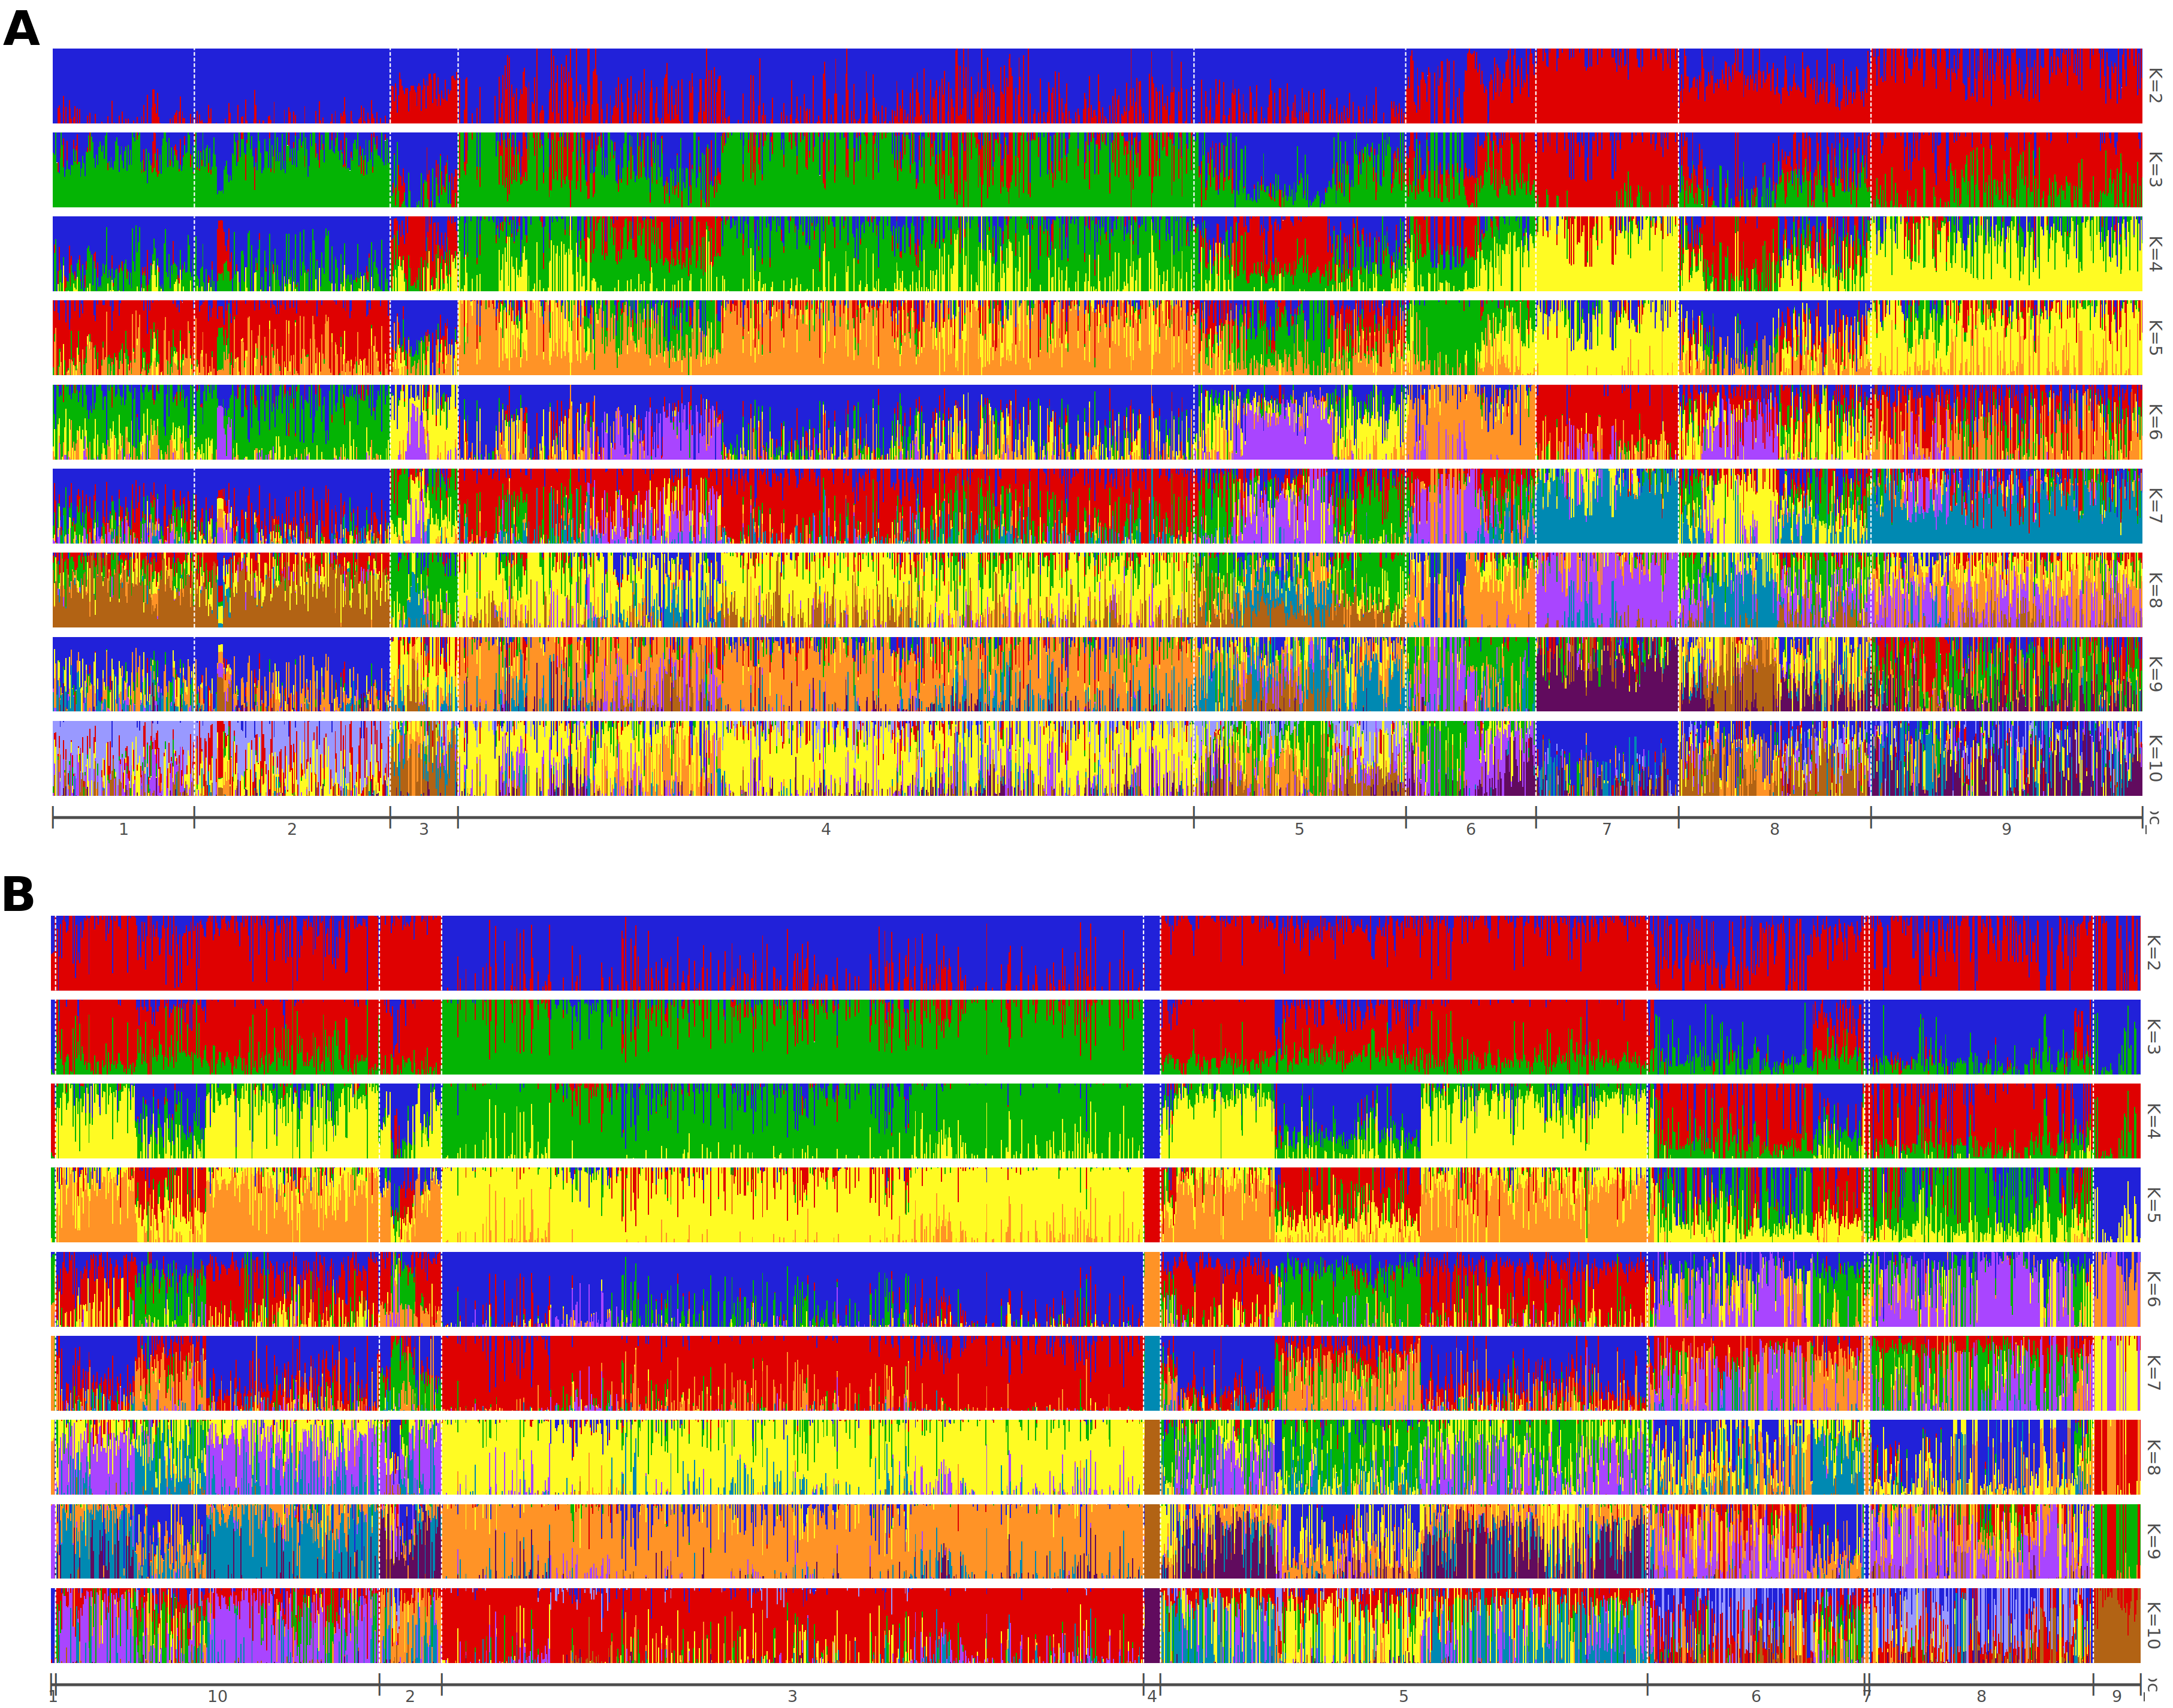
\includegraphics[width=0.9\textwidth]{./figures/admixture_Kmeans_groups.png}
\captionof{figure}{\label{admix_Kmeans}Admixture analyis of \emph{P. falciparum} samples, sorted by \emph{de novo} clusters, identified using K-means. (A) Chromosome 2 and (B) 11.}
\end{center}

\vspace{1cm}

\begin{center}
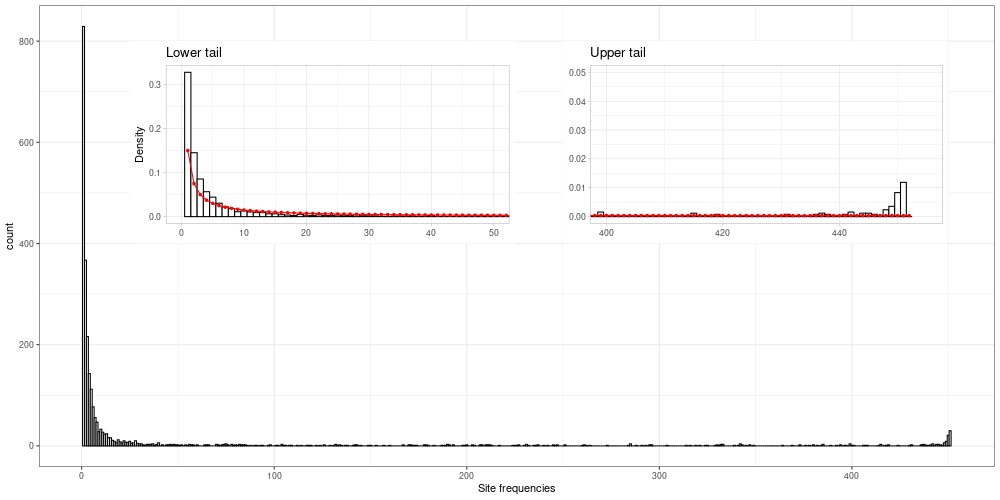
\includegraphics[width=0.9\textwidth]{./figures/sfs_unfolded_chr2_gambian_samples_unlabeled.png}
\captionof{figure}{\label{SFS_gambia}Unfolded site frequency spectrum of Gambian \emph{P. falciparum} samples.}
\end{center}

\begin{figure}[htbp]
\centering
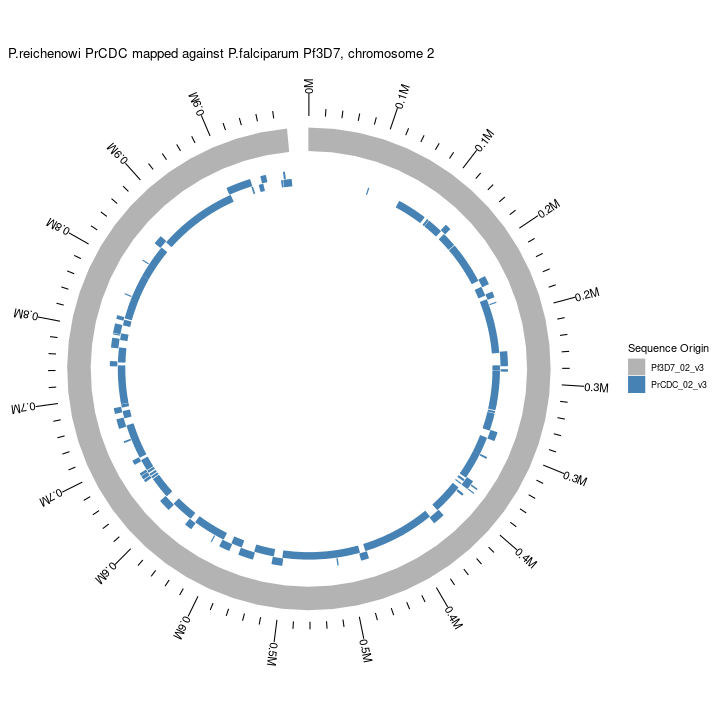
\includegraphics[width=0.6\textwidth]{./figures/Pf7_PrCDC_nucmer_chr2.png}
\caption{\label{nucmer_coverage_chr2}Mapping coverage of \emph{P. reichenowi} PrCDC aligned to the  \emph{P. falciparum} Pf3D7 reference genome (\emph{Pf7}), chromosome 2.}
\end{figure}

\begin{figure}[htbp]
\centering
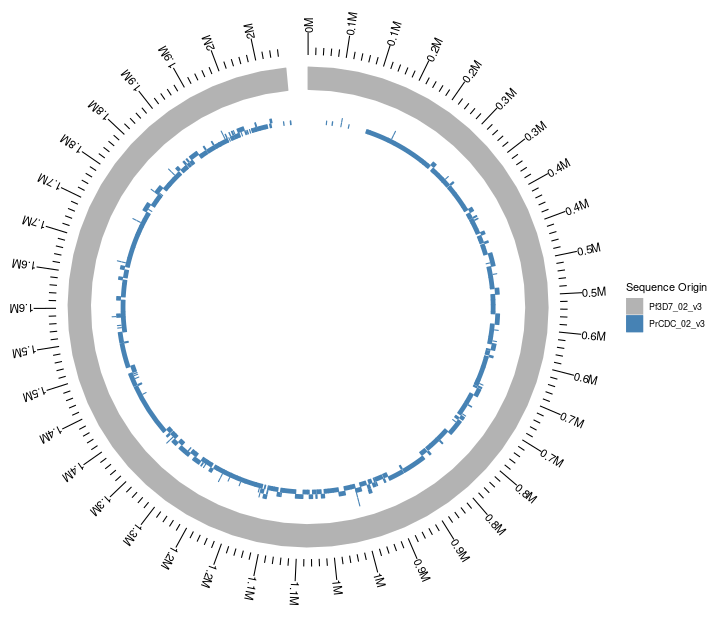
\includegraphics[width=0.6\textwidth]{./figures/Pf7_PrCDC_nucmer_chr11.png}
\caption{\label{nucmer_coverage_chr11}Mapping coverage of \emph{P. reichenowi} PrCDC aligned to the  \emph{P. falciparum} Pf3D7 reference genome (\emph{Pf7}), chromosome 11.}
\end{figure}

\subsection*{Code}
\label{sec:org5518209}
The complete code used for this report can be found in the git repository:\\[0pt]
\url{https://github.com/pwolper/Pf7-coevolution}

\subsubsection*{Filtering}
\label{sec:org30e2d82}
Downloaded VCF files where filtered and reindexed.
\begin{verbatim}
bcftools view \
    --include 'FILTER="PASS" && N_ALT=1 && TYPE="snp" && VSQLOD>5.0'\
    --samples-file $samples_dir/Pf7_african_samples_ids.txt \
    --output-type z\
    --output-file  Pf3D7_02_v3.SNP.vcf \
    Pf3D7_02_v3.pf7.vcf.gz

bcftools index -t Pf3D7_02_v3.SNP.vcf
\end{verbatim}

Heterozygous genotypes were removed using the following code as an example:
\begin{verbatim}
bcftools filter -S . -e 'GT=="het"' chr2/Pf3D7_02_v3.afr_samples.qSNP.vcf.gz\
    -o chr2/Pf3D7_02_v3.afr_samples.qSNP.GT_filtered.vcf -Oz
\end{verbatim}

\subsubsection*{DAPC}
\label{sec:orgce3ec9e}
In order to run the dapc on our vcf files we used the R package \emph{vcfR} (\cite{knaus-2017-vcfr}) to read in the file and convert it to a genlight object. Subsequently, we read in a vector of country membership and set haploidy. The dapc is conducted according to guideslines stated in \cite{thia-2022-guidel-stand}.

\begin{verbatim}
Pf7.snp <- read.vcfR(vcf_path, verbose = TRUE)

Pf7.snp.gl <- vcfR2genlight(Pf7.snp)

pop(Pf7.snp.gl) <- Pf7.metadata$Country
ploidy(Pf7.snp.gl) <- 1

clust <- find.clusters(Pf7.snp.gl, max.n.clust = 30) #de novo cluster inference
dapc <- dapc(Pf7.snp.gl, n.pca = 3, n.da = 3)
\end{verbatim}
\subsubsection*{ADMIXTURE}
\label{sec:org1f25b44}
Before converting the vcf files were converted to .bed files using \emph{plink2}, we had to rename the chromosome from Pf3D7\_x\_v3 to x. We used a names.txt file according to the bcftools documentation.

\begin{verbatim}
plink2 --vcf ../vcf/chr11/Pf3D7_11_v3.afr_samples.qSNP.GT_filtered.renamed.vcf.gz \
    --make-bed \
    --allow-extra-chr \
    -out Pf3D7_11_v3.afr_samples.qSNP.GT_filtered.renamed
\end{verbatim}

The admixture analysis was performed with the following options:
\begin{verbatim}
for K in {2..10}; do
    admixture $bed_file $K --cv | tee log{$K}.out; done
\end{verbatim}

\subsubsection*{Unfolded SFS}
\label{sec:orga6330ae}
The genome sequence of the outgroup \emph{P. reichenowi} was aligned to the \emph{P. falciparum} reference sequence Pf7 using the following code:
\begin{verbatim}
nucmer --mum -p chr11/Pf7_PrCDC \
    ../Pf7/seqs/Pf3D7_11_v3.fasta ../P.reichenowi/embl.PrCDC/PrCDC_11_v3.fasta

show-coords -c -l -r -T chr11/Pf7_PrCDC.delta > chr11/Pf7_PrCDC_coords.txt

show-snps -T chr11/Pf7_PrCDC.delta > chr11/Pf7_PrCDC_SNPs.txt

awk \
    'NR>3 && $2 !~ /\./ && $3 !~ /\./ {print}' \
    chr11/Pf7_PrCDC_SNPs.txt > chr11/Pf7_PrCDC_11_SNPs_formatted.txt
\end{verbatim}

SNP frequencies and counts were extracted with the following code:
\begin{verbatim}
bcftools query -f '%POS %REF %ALT %AF %AC %AN\n'\
    Pf3D7_02_v3.afr_samples.qSNP.GT_filtered.vcf.gz > Pf7.02.vcf.qSNP.AF_AC_AN.txt
\end{verbatim}
\end{document}